\lstset{style=pythonstyle}

\section{ТЕХНИЧЕСКАЯ РЕАЛИЗАЦИЯ И ВЕРИФИКАЦИЯ ПРОЕКТА}
\label{sec:func}

\subsection{Разработка ПО}
\label{sub:func:1}

\subsubsection{Блок пользовательского интерфейса }


Реализует интерфейс командной строки (CLI). Для обработки параметров командной строки использует пакет argparse.

Начиная с версии Python 2.7, в набор стандартных библиотек была включена библиотека argparse для обработки аргументов (параметров, ключей) командной строки. Хотелось бы остановить на ней Ваше внимание.

\begin{itemize}

	\item Для начала рассмотрим, что предлагает argparse. Argparse — это изящный инструмент для:
	\item анализа аргументов sys.argv;
	\item конвертирования строковых аргументов в объекты Вашей программы и работа с ними;
	\item форматирования и вывода информативных подсказок;
	\item многого другого.

\end{itemize}


Одним из аргументов противников включения argparse в Python был довод о том, что в стандартных модулях и без этого содержится две библиотеки для семантической обработки (парсинга) параметров командной строки. Однако, как заявляют разработчики argparse, библиотеки getopt и optparse уступают argparse по нескольким причинам:

\begin{itemize}
	\item Обладая всей полнотой действий с обычными параметрами командной строки, они не умеют обрабатывать позиционные аргументы (positional arguments). Позиционные аргументы — это аргументы, влияющие на работу программы, в зависимости от порядка, в котором они в эту программу передаются. Простейший пример — программа cp, имеющая минимум 2 таких аргумента («cp source destination»).
	\item  Argparse дает на выходе более качественные сообщения о подсказке при минимуме затрат (в этом плане при работе с optparse часто можно наблюдать некоторую избыточность кода).
	\item Argparse дает возможность программисту устанавливать для себя, какие символы являются параметрами, а какие нет. В отличие от него, optparse считает опции с синтаксисом наподобии "-pf, -file, +rgb, /f и т.п. «внутренне противоречивыми» и «не поддерживается optpars'ом и никогда не будет».
	\item Argparse даст Вам возможность использовать несколько значений переменных у одного аргумента командной строки (nargs).
	\item Argparse поддерживает субкоманды (subcommands). Это когда основной парсер отсылает к другому (субпарсеру), в зависимости от аргументов на входе.
\end{itemize}

Исходя из вышесказанного, можно сделать вывод, что argparse — довольно мощная и легкая библиотека, предоставляющая, на мой взгляд, очень удобный интерфейс для работы с параметрами командной строки.

Рассмотрим теперь реализацию интерфейса командной строки в дипломном проекте. CLI реализован при помощи класса fuzzysim.launcher.CLI.

\begin{figure}[ht]
  \centering
  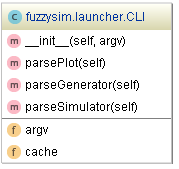
\includegraphics[scale=1]{3-1.png}
  \caption{ Структура класса fuzzysim.launcher.CLI }
  \label{fig:func:1}
\end{figure}

Поля класса fuzzisim.launcher.CLI:
\begin{itemize}
  \item \lstinline!cache!. Отображение разобранных аргументов командной строки, для дальнейшего использования.
  \item \lstinline!argv!. Список текстовых аргументов командной строки, предоставляемый оболочкой.
\end{itemize}

Методы класса fuzzisim.launcher.CLI:
\begin{itemize}
	\item  \lstinline!__init__(self, argv)!. Инициализирует поля контроллера.
	\item  \lstinline!parsePlot(self)!.  Производит разбор аргументов для визуализации графиков.
	\item  \lstinline!parseGenerator(self)!.  Производит разбор аргументов для генерации правил.
	\item  \lstinline!parseSimulator(self)!.  Производит разбор аргументов для запуска симуляции.
\end{itemize}


\subsubsection{Блок диспетчера приложения }


Блок диспетчера приложения реализован в модуле \lstinline!fuzzisim.launcher!. Он представляет из себя классический контроллер в парадигме MVC (Модель-Представление-Контроллер) и таким образом осуществляет роутинг запросов пользователя в нужный модуль. Рассмотрим его основные функции.

\paragraph{Функция generate(argv)}

 Генерирует правила для алгоритма Мамдани, анализируя собранную телеметрию, находящуюся в CSV файле. Обрабатывает параметры командной строки: --generate — имя файла с собранной телеметрией; --terms —  количество термов, на которые следует разбить область значений, --interval — флаг, показывающий, что требуется сгенерировать интервальные функции принадлежностей.

\begin{lstlisting}[style=pythonstyle,caption={ }, label=lst:func:1]
  def generate(argv):
    args = gen_parser.parse_args(argv)
    config = mamdani.generator.generate_config(args.csv_file, args.terms, args.interval)
    print(json.dumps(config, indent=4))
\end{lstlisting}

\paragraph{Функция launch(argv)}

Запускает симуляцию исходя из начальных параметров, выбранного контроллера торможения, выводит результат и собранную телеметрию. Обрабатывает параметры командной строки: distance — начальная дистанция до препятствия; speed — начальная скорость, с которой осуществляется торможение; --latency — задержки в системе управления; --way — файл конфигурации пути, содержит в себе данные о характеристиках участков пути в формате json; --controller — имя модуля контроллера торможения, который будет использоваться в симуляции; --noplot — флаг, подавляет вывод графиков собранной телеметрии; --stats — флаг, если установлен, выводит в поток стандартного вывода собранную телеметрию в формате csv вместо резюме результатов  симуляции. Если флаг --noplot не установлен, то после завершения симуляции на экран выводятся интерактивные графики с результатами симуляции.

\begin{lstlisting}[style=pythonstyle,caption={}, label=lst:func:1]
def launch(argv):
  args = sim_parser.parse_args(argv)

  simulate(
     args.distance,
     args.speed,
     args.latency,
     args.way_config_file,
     args.brake_controller,
     not args.noplot_graphs,
     args.print_stats
  )
\end{lstlisting}

\paragraph{ Функция plot(argv)}

Визуализирует результаты предварительно сохраненной телеметрии, из файла в формате CSV. В качестве аргумента принимает имя CSV файла, в котором содержится собранная телеметрия от одной или нескольких симуляций. Позволяет отображать результаты нескольких экспериментов, наложенные на один график. Кроме того, в поток стандартного вывода выводит декартово расстояние графиков экспериментов от нулевого (принимаемого за эталонный), что позволяет оценить точность вычислений.

\begin{lstlisting}[style=pythonstyle,caption={  }, label=lst:func:1]
def plot(argv):
  args = plot_parser.parse_args(argv)
  fuzzysim.charts.show_charts_csv(args.csv_file)
\end{lstlisting}


\subsubsection{Блок обучения нечетких алгоритмов }

Реализует автоматизированную генерацию термов лингвистических переменных и правил для нечетких алгоритмов. Входные данные получает в формате CSV, что обусловлено табличным характером входных данных. Источником входных данных может быть любое приложение, позволяющее представить симулированную, либо реальную телеметрию в необходимом формате. Вывод симулятора с установленным флагом -s является валидным источником данных для генератора правил.

Опишем формат входных данных. Первой строкой, завершающейся символом \\n является заголовок, в котором заданы названия колонок. Допустимые колонки:

\begin{itemize}
\item T — число с плавающей точкой, означающее количество секунд, прошедших с начала эксперимента;
\item S — число с плавающей точкой, означающее расстояние в метрах до препятствия в соответствующий момент времени эксперимента;
\item V — число с плавающей точкой, означающее текущую скорость в метрах в секунду в соответствующий момент времени эксперимента;
\item A — число с плавающей точкой, означающее текущее ускорение в метрах в секунду за секунду в соответствующий момент времени эксперимента.
\end{itemize}

Блок реализован в модуле  \lstinline!fuzzysim.mamdani.generator.! Рассмотрим его основные функции.

\paragraph{Функция generate\_config(csv\_file\_name, terms\_count, is\_interval)}

Является точкой входа в модуль. Производит разбор файла с данными, сборку объекта правил и вывод сериализованного набора правил и термов. В качестве входных аргументов принимает:

\begin{itemize}
	\item \lstinline!csv_file_name! — строка, содержащая имя CSV файла с исходными данными;
	\item \lstinline!terms_count! — целое число, количество термов, на которые разбивается пространство значений входных и выходных переменных;
	\item \lstinline!is_interval! — булево значение, показывающий требуется ли генерировать интервальные задающие функции термов.
\end{itemize}

\begin{lstlisting}[style=pythonstyle,caption={  }, label=lst:func:1]
  def generate_config(csv_file_name, terms_count, is_interval):
  data = {'S': [], 'V': [], 'A': []}

  with open(csv_file_name, newline='') as csvfile:
     reader = csv.reader(csvfile, delimiter=',', quotechar='\\\\')
     cols = {}
     for row in reader:
        if row[0] == "t":
           cols = {v.upper(): i for i, v in enumerate(row)}
           continue

        # data['T'].append(float(row[0]))
        data['S'].append(float(row[cols['S']]))
        data['V'].append(float(row[cols['V']]))
        data['A'].append(abs(float(row[cols['A']])))
     # data['J'].append(float(row[4]))

  maxs = {k: max(v) for k, v in data.items()}
  mins = {k: min(v) for k, v in data.items()}
  steps = {k: abs(maxs[k] - mins[k]) / terms_count for k, v in maxs.items()}

  config = {
     'S': get_var_config(maxs['S'], mins['S'], steps['S'], 0),
     'V': get_var_config(maxs['V'], mins['V'], steps['V'], 0),
     'A': get_var_config(maxs['A'], mins['A'], steps['A'], is_interval),
     'rules': generate_rules(data, ['S', 'V'], ['A'], terms_count)
  }

  a_map = print_map(config, terms_count)
  for s, speeds in enumerate(a_map):
     begin = True
     for v, a in enumerate(speeds):
        if a != ' ':
           begin = False
           continue

        if begin:
           # a_map[s][v] = 0
           config['rules'].append({'conds': [['S', s], ['V', v]], 'concs': [['A', 0],]})
        else:
           config['rules'].append({'conds': [['S', s], ['V', v]], 'concs': [['A', terms_count - 1],]})

  print("\\n", file=sys.stderr, sep='')
  print_map(config, terms_count)

  return config
\end{lstlisting}

\paragraph{Функция generate\_rules(data,in\_vars,out\_vars,terms\_count)}

Генерирует правила нечеткого контроллера. Определяет область значений входных и выходных переменных, разбивает их на требуемое количество термов. Затем для каждой временной точки определяет, в каким термам относятся данных значения входных и выходных переменных, и на основании этого составляется набор правил. После генерации полного набора из него удаляются дублирующиеся правила. При этом при генерации правил возможны случаи неоднозначности: при сравнительно малом количестве термов одинаковому набору входных термов может соответствовать разные наборы выходных термов. В этом случае выбирается то правило, в котором мощность множества соответствующих данному правилу срезов телеметрии максимально, однако такие ситуации обычно требуют ручной настройки правил.

В качестве входных аргументов принимает:
\begin{itemize}
	\item \lstinline!data! — многомерный массив с данными телеметрии;
	\item \lstinline!in_vars! — вектор строк, список имен входных переменных;
	\item \lstinline!out_vars! — вектор строк, список имен выходных переменных;
	\item \lstinline!terms_count! — целое число, количество термов, на которые разбивается пространство значений входных и выходных переменных.
\end{itemize}

\begin{lstlisting}[style=pythonstyle,caption={  }, label=lst:func:1]
def generate_rules(data, in_vars, out_vars, terms_count):
  rules = {}

  maxs = {k: max(v) for k, v in data.items()}
  mins = {k: min(v) for k, v in data.items()}
  steps = {k: abs(maxs[k] - mins[k]) / terms_count for k, v in maxs.items()}

  for i, _ in enumerate(list(data.values())[0]):
     terms = []
     for k, stat in data.items():
        max_term = int(abs(maxs[k] - mins[k]) / steps[k]) - 1
        terms.append([k, min(max_term, int(abs(stat[i] - mins[k]) / steps[k]))])

     in_terms = tuple(tuple(v) for v in terms if v[0] in in_vars)
     out_terms = tuple(tuple(v) for v in terms if v[0] in out_vars)

     if in_terms not in rules:
        rules[in_terms] = {}

     if out_terms not in rules[in_terms]:
        rules[in_terms][out_terms] = 0

     rules[in_terms][out_terms] += 1

  # rules[in_terms] = out_terms

  return list([{'conds': k, 'concs': max(v.items(), key=lambda x: x[1])[0]} for k, v in rules.items()])
\end{lstlisting}

\paragraph{Функция print\_map(config, terms\_count)}

Выводит визуализацию сгенерированных правил. Печатает в поток стандартного вывода матрицу правил, где номер строки соответствует номеру терма расстояния, а номер столбца — номеру терма скорости. Значение элемента — номер терма ускорения.

В качестве входных аргументов принимает:
\begin{itemize}
	\item \lstinline!config! — объект с правилами и термами;
	\item \lstinline!terms_count! — целое число, количество термов, на которые разбивается пространство значений входных и выходных переменных.
\end{itemize}

\begin{lstlisting}[style=pythonstyle,caption={  }, label=lst:func:1]
def print_map(config, terms_count):
  a_map = []
  for i in range(0, terms_count):
     a_map.append([])
     for j in range(0, terms_count):
        a_map[i].append(' ')

  for r in config['rules']:
     m = {}
     for c in r['conds']:
        m[c[0]] = c[1]
     v = str(r['concs'][0][1])
     a_map[m['S']][m['V']] = v

  print('S\\V', [str(i) for i in range(0, terms_count)], file=sys.stderr, sep='')
  for i, row in enumerate(a_map):
     print("%03d" % i, row, file=sys.stderr, sep='')

  return a_map
\end{lstlisting}

\subsubsection{ Блок визуализации телеметрии}


Осуществляет представление собранной телеметрической информации в виде интерактивных графиков и реализован в модуле fuzzysim.charts.

Графики выводятся при помощи пакета \lstinline!Matplotlib!, который позволяет изменять масштаб, сохранять скриншоты, просмотреть точные значения в различных точках графика.  \lstinline!Matplotlib! является де-факто стандартом для визуализации научных данных.

\lstinline!Matplotlib! состоит из множества модулей. Модули наполнены различными классами и функциями, которые иерархически связаны между собой.

Создание рисунка в \lstinline!matplotlib! схоже с рисованием в реальной жизни. Так художнику нужно взять основу (холст или бумагу), инструменты (кисти или карандаши), иметь представление о будущем рисунке (что именно он будет рисовать) и, наконец, выполнить всё это и нарисовать рисунок деталь за деталью.

В \lstinline!matplotlib! все эти этапы также существуют, и в качестве художника-исполнителя здесь выступает сама библиотека. От пользователя требуется управлять действиями художника-\lstinline!matplotlib!, определяя что именно он должен нарисовать и какими инструментами. Обычно создание основы и процесс непосредственно отображения рисунка отдаёт полностью на откуп \lstinline!matplotlib!. Таким образом, пользователь библиотеки \lstinline!matplotlib! выступает в роли управленца. И чем проще ему управлять конечным результатом работы \lstinline!matplotlib!, тем лучше.

Так как \lstinline!matplotlib! организована иерархически, а наиболее простыми для понимания человеком являются самые высокоуровневые функции, то знакомство с \lstinline!matplotlib! начинают с самого высокоуровневого интерфейса \lstinline!matplotlib.pyplot!. Так, чтобы нарисовать гистограмму с помощью этого модуля, нужно вызывать всего одну команду: m\lstinline!atplotlib.pyplot.hist(arr)!.

Пользователю не нужно думать как именно библиотека нарисовала эту диаграмму. Если бы мы рисовали гистограмму самостоятельно , то заметили бы, что она состоит из повторяющихся по форме фигур - прямоугольников. А чтобы нарисовать прямоугольник, нужно знать хотя бы координату одного угла и ширину/длину. Рисовали же бы мы прямоугольник линиями, соединяя угловые точки прямоугольника.

В тоже время для более серьёзных задач (внедрение \lstinline!matplotlib! в пользовательскую GUI) требуется больше контроля над процессом и больше гибкости, чем могут предоставить эти два модуля. Необходим доступ к более низкоуровневым возможностям библиотеки, которая реализована в объектно-ориентированном стиле. ООС заметно сложнее для новичков и требует знаний о работе конкретных классов и их методах, но предоставляет самые большие возможности по взаимодействию с библиотекой \lstinline!matplotlib!.

Главной единицей (объектом самого высокого уровня) при работе с \lstinline!matplotlib! является рисунок (\lstinline!Figure!). Любой рисунок в \lstinline!matplotlib! имеет вложенную структуру и чем-то напоминает матрёшку:

\begin{itemize}
	\item  \textit{Рисунок (\lstinline!Figure!)}. Рисунок является объектом самого верхнего уровня, на котором располагаются одна или несколько областей рисования (\lstinline!Axes!), элементы рисунка \lstinline!Artisits! (заголовки, легенда и т.д.) и основа-холст (Canvas). На рисунке может быть несколько областей рисования \lstinline!Axes!, но данная область рисования \lstinline!Axes! может принадлежать только одному рисунку \lstinline!Figure!.
	\item  \textit{Область рисования (\lstinline!Axes!)}. Область рисования является объектом среднего уровня, который является, наверное, главным объектом работы с графикой \lstinline!matplotlib! в объектно-ориентированом стиле. Это то, что ассоциируется со словом <<\lstinline!plot!>>, это часть изображения с пространством данных. Каждая область рисования \lstinline!Axes! содержит две (или три в случае трёхмерных данных) координатных оси (\lstinline!Axis! объектов), которые упорядочивают отображение данных.
	\item  \textit{Координатная ось (\lstinline!Axis!)}. Координатная ось являются объектом среднего уровня, которые определяют область изменения данных, на них наносятся деления \lstinline!ticks! и подписи к делениям \lstinline!ticklabels!. Расположение делений определяется объектом \lstinline!Locator!, а подписи делений обрабатывает объект \lstinline!Formatter!. Конфигурация координатных осей заключается в комбинировании различных свойств объектов \lstinline!Locator! и \lstinline!Formatter!.
	\item  \textit{Элементы рисунка (\lstinline!Artists!)}. Элементы рисунка Artists являются как бы красной линией для всех иерархических уровней. Практически всё, что отображается на рисунке является элементом рисунка , даже объекты \lstinline!Figure!, \lstinline!Axes! и \lstinline!Axis!. Элементы рисунка \lstinline!Artists! включают в себя такие простые объекты как текст (\lstinline!Text!), плоская линия (\lstinline!Line2D!), фигура (\lstinline!Patch!) и другие.
\end{itemize}

Когда происходит отображение рисунка, все элементы рисунка \lstinline!Artists! наносятся на основу-холст. Большая часть из них связывается с областью рисования \lstinline!Axes!. Также элемент рисунка не может совместно использоваться несколькими областями Axes или быть перемещён с одной на другую.

В \lstinline!matplotlib! изобразительные функции логически разделены между несколькими объектами, причём каждый из них сам имеет довольно сложную структуру. Можно выделить три уровня интерфейса прикладного программирования(\lstinline!matplotlib! API):

\begin{itemize}
	\item  \lstinline!matplotlib.backend_bases.FigureCanvas! — абстрактный базовый класс, который позволяет рисовать и визуализировать результаты команд.
	\item  \lstinline!matplotlib.backend_bases.Renderer !— объект (абстрактный класс), который знает как рисовать на \lstinline!FigureCanvas!;
	\item  \lstinline!matplotlib.artist.Artist! — объект, который знает, как использовать визуализатор, чтобы рисовать на холсте.
\end{itemize}


\lstinline!FigureCanvas! и \lstinline!Renderer! обрабатывают детали, необходимые для взаимодействия со средствами пользовательского интерфейса, так как это делает \lstinline!WxPython! или язык рисования \lstinline!PostScript!. А \lstinline!Artist! обрабатывает все конструкции высокого уровня такие как представление и расположение рисунка, текста и линий.

Существует два типа объектов-классов \lstinline!Artists!: примитивы и контейнеры.

Примитивы представляют собой стандартные графические объекты: плоскую линию, прямоугольник, текст, изображение и т.д. А контейнеры - это объекты-хранилища, на которые можно наносить графические примитивы. К контейнерам относятся рисунок, область рисования, координатная ось деления. Рассмотрим контейнеры подробнее, так как именно с помощью обращений к различным контейнерам класса Artists, объединенных логически в единую структуру, будет осуществляться пользовательская настройка рисунков в \lstinline!matplotlib!.

Всего существует 4 вида \lstinline!Artists! контейнеров:

\begin{itemize}
	\item  Контейнеры рисунка. \lstinline!Figure! - это контейнер самого высокого уровня. На нём располагаются все другие контейнеры и графические примитивы.

	\item  Контейнеры областей рисования. \lstinline!Axes! - очень важный контейнер, так как именно с ним чаще всего работает пользователь. Экземпляры \lstinline!Axes! - это области, располагающиеся в контейнере \lstinline!Figure!, для которых можно задавать координатную систему (декартовая или полярная). На нём располагаются все другие контейнеры, кроме \lstinline!Figure!, и графические примитивы. Это области на рисунке, на которых располагаются графики и диаграммы, в которые вставляются изображения и т.д. Мультиоконные рисунки состоят из набора областей \lstinline!Axes!.

	\item  Контейнеры осей. \lstinline!Axis! похож на \lstinline!Axes! по названию, но не стоит их путать. Этот контейнер обслуживает экземпляры Axes. Он отвечает за создание координатных осей, на которые будут наноситься деления осей, подписи делений и линий вспомогательной сетки. Его специализация (и отличие от контейнера \lstinline!Tick!) - это расположение делений и линий, их позиционирование и форматирование подписей делений, их отображение.

	\item  Контейнеры делений. Контейнер низшего уровня. Его специализация (и отличие от контейнера \lstinline!Axis!) - задавать характеристики (цвет, толщина линий) линий сетки, делений и их подписей (размеры и типы шрифтов).
\end{itemize}

При создании рисунка в \lstinline!matplotlib! обычно поступают так: создают экземпляр класса \lstinline!Figure!, на котором выделяют одну или нескольких областей \lstinline!Axes!, и используют вспомогательные методы экземпляра класса \lstinline!Axes! для создания графических примитивов. Если автоматически подобранные характеристики координатной сетки, делений и их подписей не устраивают пользователя, то они настраиваются с помощью экземпляров контейнеров \lstinline!Axis! и \lstinline!Tick!, которые всегда присутствуют на созданной области рисования \lstinline!Axes!.

Опишем основные функции модуля \lstinline!fuzzysim.charts!.

\paragraph{Функция show\_charts\_csv(csv\_file\_name, terms\_count, is\_interval)}

Является основной точкой входа в модуль. На первом этапе работы разбирает входной файл данных:

\begin{lstlisting}[style=pythonstyle,caption={  }, label=lst:func:1]
experiments = []
experiment = None
with open(csv_file_name, newline='') as csvfile:
  reader = csv.reader(csvfile, delimiter=',', quotechar='\\')
  for row in reader:
     if row[0] == "t":
        # new experiment
        if experiment is not None:
           experiments.append(experiment)
        experiment = {'stats_t': [], 'stats_s': [], 'stats_v': [], 'stats_a': [], 'stats_j': []}
        continue

     experiment['stats_t'].append(float(row[0]))
     experiment['stats_s'].append(float(row[1]))
     experiment['stats_v'].append(float(row[2]))
     experiment['stats_a'].append(float(row[3]))
     experiment['stats_j'].append(float(row[4]))

experiments.append(experiment)
\end{lstlisting}


В качестве входного аргумента получает строку с именем CSV файла данных. Данные для визуализации получает в формате CSV, что обусловлено табличным характером входных данных. Источником входных данных может быть любое приложение, позволяющее представить симулированную, либо реальную телеметрию в необходимом формате. Вывод симулятора с установленным флагом “-s” является валидным источником данных для генератора правил.

Опишем формат входных данных. Первой строкой, завершающейся символом \\n является заголовок, в котором заданы названия колонок. Допустимые колонки:

\begin{itemize}
	\item T — число с плавающей точкой, означающее количество секунд, прошедших с начала эксперимента;
	\item S — число с плавающей точкой, означающее расстояние в метрах до препятствия в соответствующий момент времени эксперимента;
	\item V — число с плавающей точкой, означающее текущую скорость в метрах в секунду в соответствующий момент времени эксперимента;
	\item A — число с плавающей точкой, означающее текущее ускорение в метрах в секунду за секунду в соответствующий момент времени эксперимента.
\end{itemize}

После разбора CSV файла происходит группировка табличных данных в датасеты, разбитые по экспериментам:

\begin{lstlisting}[style=pythonstyle,caption={  }, label=lst:func:1]
datasets = []
for en, experiment in enumerate(experiments):
  experiment_datasets = get_datasets(**experiment)

  for i, ds in enumerate(experiment_datasets):
     if i == len(datasets):
        datasets.append({'sub': []})

     datasets[i]['xl'] = ds['xl']
     datasets[i]['yl'] = ds['yl']
     ds['yl'] = "(%d) %s" % (en, ds['yl'])
     datasets[i]['sub'].append(ds)
\end{lstlisting}

После этого вызываются функции вывода статистики и отображения графиков.

\paragraph{Функция show\_stats(experiments)}

Выводит в поток стандартного вывода декартово расстояние между нулевым экспериментом и каждым другим, встречающимся в входном файле. В качестве входного параметра принимает массив структур experiment, содержащих сгруппированные данных из входного файла.

\begin{lstlisting}[style=pythonstyle,caption={  }, label=lst:func:1]
  def show_stats(experiments):
  if len(experiments) < 2:
     return

  gauge = experiments[0]
  stats = {'stats_s':{}, 'stats_v':{}, 'stats_a':{}, 'stats_j':{}}
  for en, experiment in enumerate(experiments):
     for param in stats:
        sum = 0
        for i, s in enumerate(experiment[param]):
           G = len(gauge[param]) > i and gauge[param][i] or 0
           sum += (s - G)**2
        sum /= len(experiment[param])
        stats[param][en] = math.sqrt(sum)

  print("Normalized quadratic Parameters deviations by experiment:")
  pprint.pprint(stats)
\end{lstlisting}



\paragraph{Функция plot\_datasets(datasets)}

    Отображает данные датасетов при помощи пакета модуля \lstinline!matplotlib.pyplo!t. Она автоматически формирует легенду, добавляет подписи к к осям, формирует заголовки страниц. При этом графики разбиваются на типы в соответствии с данными датасетов, и на один график накладываются данные разных экспериментов, что позволяет их сравнивать. Для одновременного отображения разных графиков используются \lstinline!pyplot figures! (рисунки):

Рисунок - это общее окно или страница, на которой все нарисовано. Это компонент верхнего уровня всех тех, которые вы рассмотрите в следующих пунктах. Вы можете создать несколько независимых фигур. На рисунке может быть несколько других вещей, таких как \lstinline!suptitle!, который является центральным названием фигуры. Вы также обнаружите, что вы можете добавить легенду и цветную панель, например, к вашей фигуре.

К фигуре добавляются оси. Оси - это область, на которой построены данные с такими функциями, как \lstinline!plot()! и \lstinline!scatter()!, и которые могут иметь связанные с ней клещи, метки и т. Д. Это объясняет, почему фигуры могут содержать несколько осей.

Когда вы хотите просмотреть свои сюжеты на вашем дисплее, бэкэнду пользовательского интерфейса нужно будет запуститься \lstinline!GUI mainloop!. Это то, что делает \lstinline!show()!. Он сообщает \lstinline!Matplotlib!, чтобы поднять все окна с фигурами, созданные до сих пор, и запустить \lstinline!mainloop!. Поскольку этот \lstinline!mainloop! блокируется по умолчанию (т.е. выполнение скрипта приостановлено), вы должны только вызывать его один раз для каждого скрипта, в конце. Выполнение скрипта возобновляется после закрытия последнего окна.

Приведем часть кода функции \lstinline!plot_datasets(datasets)!

\begin{lstlisting}[style=pythonstyle,caption={  }, label=lst:func:1]
def plot_datasets(datasets):

  for ds in datasets:
     (f, ax) = plt.subplots()

     ax.grid(True)

#     <...>

     if 'sub' in ds:
        for sub in ds['sub']:

           label = 'yl' in sub and sub['yl']
           marker = 'ym' in sub and sub['ym'] or None
           ax.plot(sub['x'], sub['y'], label=label, marker=marker)
           ax.legend()

     ax.spines['left'].set_position('zero')
     ax.spines['bottom'].set_position('zero')
     ax.spines['left'].set_smart_bounds(True)
     ax.spines['bottom'].set_smart_bounds(True)

  plt.show()
\end{lstlisting}

\paragraph{Функция show\_charts\_simulation(simulator)}

Отображает графики эксперимента непосредственно после симуляции, поэтому не требует разбора CSV файла. В качетсве входного параметра принимает объект симулятора класса \lstinline!fuzzysim.Simulator! и собирает телеметрию из него.

\begin{lstlisting}[style=pythonstyle,caption={  }, label=lst:func:1]
def show_charts_simulator(simulator):
  """
  Prepare datasets and plot it
  """
  stats_t, stats_s, stats_v, stats_a, stats_j = simulator.stats_t, simulator.stats_s, simulator.stats_v, simulator.stats_a, simulator.stats_j
  datasets = get_datasets(stats_t, stats_s, stats_v, stats_a, stats_j)
  plot_datasets(datasets)
\end{lstlisting}

\paragraph{Функция show\_vars(alg: mamdani.MamdaniAlgorithm)}

Отображает графики функций принадлежности входных и выходных лингвистических переменных для алгоритмов мамдани, принимая в качестве входного аргумента экземпляр класса fi. Из него извлекаются входные и выходные переменные, и по ним строятся графики принадлежностей.

\begin{lstlisting}[style=pythonstyle,caption={  }, label=lst:func:1]
def show_vars(alg: mamdani.MamdaniAlgorithm):
  f = plt.figure(1)
  f.suptitle("Out variables")
  setup_variables(alg.in_variables.values())

  f = plt.figure(2)
  f.suptitle("In Variables")
  setup_variables(alg.out_variables.values())

  plt.show()
\end{lstlisting}

\paragraph{Функция setup\_variables(variables)}

Является вспомогательной для \lstinline!show_vars()! и извлекает точки экстремума из объектов лингвистических переменных для отображения графика, а также формирует подписи к графикам и легенде.

\begin{lstlisting}[style=pythonstyle,caption={  }, label=lst:func:1]
def setup_variables(variables):
  for i, variable in enumerate(variables):
     ax = plt.subplot(len(variables), 1, i+1)
     ax.grid(True)
     ax.set_title("Variable: %s" % variable.name, loc='left')
     ax.spines['bottom'].set_position('zero')
     ax.spines['left'].set_position('zero')

     for t in variable.terms.values():
        c = min(t.c, variable.max)
        d = min(t.d, variable.max)
        plt.plot([t.a, t.b, c, d], [0, t.height, t.height, 0])
\end{lstlisting}

\subsubsection{Блок симуляции  }


Блок симуляции реализован в классе модулем \lstinline!fuzzysim.fuzzysim.Simulator!. Данный блок контролирует подсистемы симуляции физической модели, контроллера платформы, конфигурации пути, сбора телеметрии. Он инициализирует вышеуказанные системы перед началом симуляции, задает такты модельного времени, хранит собранную телеметрию.

Является фасадом для остальных частей системы. Агрегирует экземпляр класса физической модели и экземпляр класса контроллера платформы.

При проектировании сложных систем, зачастую применяется т.н. принцип декомпозиции, при котором сложная система разбивается на более мелкие и простые подсистемы. Причем, уровень декомпозиции (ее глубину) определяет исключительно проектировщик. Благодаря такому подходу, отдельные компоненты системы могут быть разработаны изолированно, затем интегрированы вместе. Однако возникает, очевидная на первый взгляд, проблема — высокая связность модулей системы. Это проявляется, в первую очередь, в большом объеме информации, которой модули обмениваются друг с другом. К тому же, для подобной коммуникации одни модули должны обладать достаточной информацией о природе других модулей.

Таким образом, минимизация зависимости подсистем, а также снижение объема передаваемой между ними информации — одна из основных задач проектирования.

Паттерн «Фасад» предоставляет унифицированный интерфейс вместо набора интерфейсов некоторой подсистемы. Фасад определяет интерфейс более высокого уровня, который упрощает использование подсистемы.

Проще говоря, «Фасад» — есть ни что иное, как некоторый объект, аккумулирующий в себе высокоуровневый набор операций для работы с некоторой сложной подсистемой. Фасад агрегирует классы, реализующие функциональность этой подсистемы, но не скрывает их. Важно понимать, что клиент, при этом, не лишается более низкоуровневого доступа к классам подсистемы, если ему это, конечно, необходимо. Фасад упрощает выполнение некоторых операций с подсистемой, но не навязывает клиенту свое использование.

\begin{figure}[ht]
  \centering
  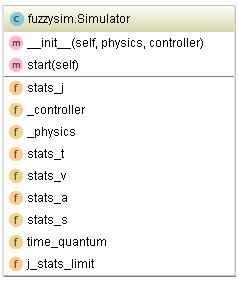
\includegraphics[scale=1]{3-2.png}
  \caption{ Структура класса fuzzisim.fuzzisim.Simulator}
\end{figure}

Поля класса fuzzisim.fuzzisim.Simulator:
\begin{itemize}
	\item \lstinline!_controller!. Контроллер платформы. Выдает управляющие сигналы на торможение.
	\item \lstinline!_physics!. Физическая модель. Рассчитывает скорость платформы, ее ускорение, рывок и положение в текущий момент модельного времени исходя из управляющих сигналов, поданных контроллером платформы, задержек в системе управления  и характеристиками пути.
	\item \lstinline!time_quantum!. Величина одного кванта модельного времени, в секундах. Исходя из нее устанавливаются размеры квантов времени физической модели и контроллера платформы.
	\item \lstinline!j_stats_limit!. Максимальное значение рывка, которое следует учитывать при сборе телеметрии.
	\item \lstinline!stats_t!. Массив со значениями модельного времени в секундах, относящемуся к текущему срезу телеметрии.
	\item \lstinline!stats_s!. Массив со значениями расстояния до препятствия в метрах, относящемуся к текущему срезу телеметрии.
	\item \lstinline!stats_v!. Массив со значениями скорости в метрах в секунду, относящемуся к текущему срезу телеметрии.
	\item \lstinline!stats_a!. Массив со значениями ускорения в метрах в секунду за секунду, относящемуся к текущему срезу телеметрии.
	\item \lstinline!stats_j!. Массив со значениями рывка в метрах в секунду за секунду за секунду, относящемуся к текущему срезу телеметрии.
\end{itemize}

Методы класса fuzzisim.fuzzisim.Simulator:
\begin{itemize}
  \item \lstinline!__init__(self, physics, controller)! — конструктор, инициализирует поля и классы-делегаты. В качестве аргументов принимает объекты физической модели и контроллера платформы.
  \item \lstinline!start(self)! — запускает симуляцию, генерирует такты модельного времени, собирает телеметрию, а также детектирует окончание симуляции по причине остановки платформы, либо ее столкновения с препятствием.
\end{itemize}

\begin{lstlisting}[style=pythonstyle,caption={  }, label=lst:func:1]
lass Simulator:
  """
  Manage controllers, generate ticks, collects stats
  """
  time_quantum = 0.001
  j_stats_limit = 100

  def __init__(self, physics, controller):
     """
     Inits world

     :param physics: PhysModel
     :param controller: CartController
     """
     physics.time_quantum = self.time_quantum
     controller.time_quantum = self.time_quantum

     self._physics = physics
     self._controller = controller

     self.stats_t = []
     self.stats_s = []
     self.stats_v = []
     self.stats_a = []
     self.stats_j = []

  def start(self):
     prev_a = 0
     while not self._physics.is_stopped():
        try :
           self._physics.tick()
        except CollisionError as e:
           return False, e.t, e.s, e.v, e.a

        self._controller.tick()

        (t, s, v, a) = self._physics.get_params()

        j = (a - prev_a) / (self.time_quantum)
        j = math.copysign(min(abs(j), self.j_stats_limit), j)
        prev_a = a

        self.stats_t.append(t)
        self.stats_s.append(s)
        self.stats_v.append(v)
        self.stats_a.append(a)
        self.stats_j.append(j)

     return True, t, s, v, a
\end{lstlisting}

\subsubsection{ Блок физической модели}

Блок физической модели реализован модулем \lstinline!fuzzysim.fuzzysim!. Данный блок состоит из следующих классов:

\begin{itemize}
	\item \lstinline!fuzzisim.fuzzisim.PhysModel;!
	\item \lstinline!fuzzisim.fuzzisim.CartController;!
	\item \lstinline!fuzzisim.fuzzisim.WayConfig;!
	\item \lstinline!fuzzisim.fuzzisim.Obstacle;!
	\item \lstinline!fuzzisim.fuzzisim.CollisionError.!
\end{itemize}

\paragraph{fuzzisim.fuzzisim.PhysModel}

Реализует физическую модель симуляции. Рассчитывает скорость платформы, ее ускорение, рывок и положение в текущий момент модельного времени исходя из управляющих сигналов, поданных контроллером платформы, задержек в системе управления и характеристиками пути.

\begin{figure}[ht]
    \centering
    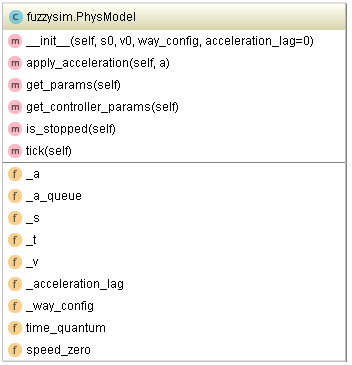
\includegraphics[scale=0.8]{3-3.png}
    \caption{  Структура класса fuzzisim.fuzzisim.PhysModel }
    \label{fig:domain:1:1}
\end{figure}

Поля класса \lstinline!fuzzisim.fuzzisim.PhysModel!:

\begin{itemize}
	\item  \lstinline!_a!. Текущее фактическое ускорение в метрах в секунду за секунду.
	\item  \lstinline!_a_queue!. Очередь управляющих сигналов контроллера платформы, устанавливающих ускорение. Применяется для окрректной обработки задержек в системе торможения.
	\item  \lstinline!_s!. Текущее расстояние для препятствия, в метрах.
	\item  \lstinline!_t!. Текущий момент модельного времени, в секундах.
	\item  \lstinline!_v!. Текущая скорость, в метрах в секунду.
	\item  \lstinline!_acceleration_lag!. Величина задержки в системе торможения, в секундах.
	\item  \lstinline!_way_config!. Конфигурация пути. Представлена экземпляром класса fuzzisim.fuzzisim.WayConfig. Используется для определения предельных ускорений на данном участке пути, а также для определения дополнительных сил, действующих на платформу.
	\item  \lstinline!time_quantum!. Величина одного кванта модельного времени, в секундах.
	\item  \lstinline!speed_zero!. Значение скорости в метрах в секунду, при котором платформа считается остановившейся.
\end{itemize}
Методы класса \lstinline!fuzzisim.fuzzisim.PhysModel!:
\begin{itemize}
	\item  \lstinline!__init__(self, s0, v0, way_config, acceleration_lag=0)!. Инициализирует физическую модель . В качестве входных аргументов принимает начальную скорость платформы в метрах в секунду, начальное расстояние до препятствия в метрах, объект конфигурации пути, значение задержек в системе управления в секундах. начальный момент времени и начальное ускорения принимаются равными нулю.
	\item  \lstinline!apply_acceleration(self, a)!. Предоставляет интерфейс контроллеру платформы, позволяющий послать физической модели управляющий сигнал, на изменение ускорения. В качестве входного параметра принимает значение ускорения в метрах в секунду за секунду
	\item  \lstinline!get_params(self)!. Предоставляет интерфейс менеджеру симуляции для сбора телеметрии, Возвращает кортеж значений (\lstinline!t, s, v, a!): значения текущей метки времени в секундах, расстояния до препятствия в метрах, скорости в метрах в секунду, ускорения в метрах в секунду за секунду.
	\item  \lstinline!get_controller_params(self)!. Предоставляет интерфейс контроллеру платформы, позволяющий получить симулированные зданные от внешних датчиков расстояния, скорости и ускорения. Возвращает кортеж значений (\lstinline!s, v, a!): значения расстояния до препятствия в метрах, скорости в метрах в секунду, ускорения в метрах в секунду за секунду
	\item  \lstinline!is_stopped(self)!. Возвращает истину в случае, если скорость платформы меньше \lstinline!speed_zero!
	\item  \lstinline!tick(self)!.  Осуществляет рассчет состояния системы в следующий квант времени.
\end{itemize}



\begin{lstlisting}[style=pythonstyle,caption={  }, label=lst:func:1]
def tick(self):
  """
  process tick

  :return: True if platform stopped in this quant
  """
  self._t += self.time_quantum

  # apply a from queue
  for i, v in enumerate(self._a_queue):
     if v[0] <= self._t:
        self._a = v[1]
        del self._a_queue[i]

  self._a = self._way_config.get_effective_a(self._s, self._a)

  self._v += self._a * self.time_quantum
  self._s -= self._v * self.time_quantum + (self._a * self.time_quantum ** 2) / 2

  if self._s <= 0 and not self.is_stopped():
     raise CollisionError(self._t, self._s, self._v, self._a)

  # if distance less then 1 quantum zero speed distance, assume it is 0
  if abs(self._s) < self.time_quantum * self.speed_zero:
     self._s = 0
\end{lstlisting}

\paragraph{fuzzisim.fuzzisim.CartController}


Реализует модель контроллера платформы, при этом алгоритм расчета ускорения делегируется модулю \lstinline!brake_controller!. При этом используется шаблон проектирования <<стратегия>>.

Паттерн стратегия является настолько распространенным и общепринятым, что многие его используют постоянно, даже не задумываясь о том, что это хитроумный паттерн проектирования, расписанный когда-то GOF.

Каждый второй раз, когда мы пользуемся наследованием, мы используем Стратегию; каждый раз, когда мы абстрагируемся от некоторого процесса, поведения или алгоритма – мы используем стратегию. Сортировка, анализ данных, валидация, разбор данных, сериализация, кодирование, получение конфигурации, все эти концепции могут и должны быть выражены в виде стратегии или политики (policy).

Стратегия является фундаментальным паттерном, поскольку она проявляется в большинстве других классических паттернов, которые поддерживают специализацию за счет наследования. Абстрактная фабрика – это стратегия создания семейства объектов; фабричный метод – стратегия создания одного объекта; строитель – стратегия построения объекта; итератор – стратегия перебора элементов и т.д.

При этом мы не хотим, чтобы анализатор паттернов (PatternsAnalyzer) знал, какая конкретно стратегия определения паттернов используется, поэтому вместо использования конкретного типа, анализатор будет принимать детектор через аргументы конструктора. Таким образом мы не просто абстрагируемся от процесса определения паттернов, но и позволяем клиентскому коду, который использует анализатор паттернов определять стратегию самостоятельно.

По определению, применение стратегии обусловлено двумя причинами:  инкапсуляция поведения или алгоритма и  возможность замены поведения или алгоритма во время исполнения. Любой нормально спроектированный класс уже инкапсулирует в себе поведение или алгоритм, но не любой класс с некоторым поведением является или должен быть стратегией. Стратегия нужна тогда, когда важно иметь возможность заменить его во время исполнения!

Другими словами, стратегия обеспечивает точку расширения системы в определенной плоскости: класс-потребитель стратегии не знает, как выполняется некоторое действие и кто именно его выполняет; об этом знают классы более высокого уровня.

\begin{figure}[ht]
	\centering
	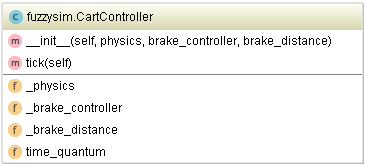
\includegraphics[scale=0.8]{3-4.png}
	\caption{ Структура класса fuzzisim.fuzzisim.CartController }
	% \label{fig:func:1}
\end{figure}

Поля класса fuzzisim.fuzzisim.CartConrtoller:
\begin{itemize}
	\item  \lstinline!_physics!. Объект физической модели, требуется для получения алгоритмом данных о расстоянии, скорости и ускорении от стимулированных датчиков.
	\item  \lstinline!_brake_controller!. Стратегия алгоритма торможения, подпакет пакета f\lstinline!uzzysim.brake_controller!.
	\item  \lstinline!_brake_distance!. Расстояние от препятствия в метрах, на котором надо затормозить.
\end{itemize}
Методы класса fuzzisim.fuzzisim.CartController:
\begin{itemize}
	\item  \lstinline!__init__(self, physics, brake_controller, brake_distance)!. Инициализирует поля контроллера.
	\item  \lstinline!tick(self)!.  Вызывает выполнение алгоритма торможения для следующего кванта времени.
\end{itemize}


\paragraph{fuzzisim.fuzzisim.WayConfig}

Класс \lstinline!fuzzisim.fuzzisim.WayConfig! реализует характеристики пути: максимальное применимое ускорение и добавочное ускорение на отдельных участках пути. Это позволяет симулировать области с пониженным коэффициентом сцепления с дорогой, ветер, подъемы и спуски. Участки  с разными характеристиками могут накладываться друг на друга, в этом случае их параметры применяются последовательно. При этом сначала применяется первый описанный участок пути, затем второй и так далее.

\begin{figure}[ht]
	\centering
	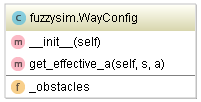
\includegraphics[scale=0.8]{3-5.png}
	\caption{ Структура класса fuzzisim.fuzzisim.WayConfig}
	% \label{fig:func:1}
\end{figure}

Поля класса fuzzisim.fuzzisim.WayConfig:
\begin{itemize}
	\item \lstinline! _obstacles!. Массив объектов класса Obstacle, описывающих конфигурацию пути.
\end{itemize}
Методы класса fuzzisim.fuzzisim.WayConfig:
\begin{itemize}
	\item \lstinline! __init__(self)!. Инициализирует поля контроллера.
	\item \lstinline! get_effective_a(self, s, a)!.  Рассчитывает эффективное ускорение в данной точке пути с учетом всех имеющихся участков. Входные аргументы: расстояние до препятствия в метрах, применяемое ускорение в метрах в секунду за секунду. Выходные параметры: рассчитанное эффективное ускорение в метрах в секунду за секунду.
\end{itemize}

\begin{lstlisting}[style=pythonstyle,caption={  }, label=lst:func:1]
def get_effective_a(self, s, a):

	for o in self._obstacles:
		a = o.get_effective_a(s, a)

	return a
\end{lstlisting}




\paragraph{fuzzisim.fuzzisim.Obstacle}

Реализует параметры конкретного участка пути. Позволяет устанавливать следующие параметры:
\begin{itemize}
	\item \lstinline! !Границы участка. Отметки расстояния от точки торможения, задающие конфигурируемый участок.
	\item \lstinline! !Константное добавочное ускорение. Позволяет моделировать наклонные участки пути.
	\item \lstinline! !Максимальное применяемое ускорение. Позволяет моделировать ограничения коэффициента сцепления с дорогой: обледенелые, мокрые, изношенные участки пути.
\end{itemize}

\begin{figure}[ht]
	\centering
	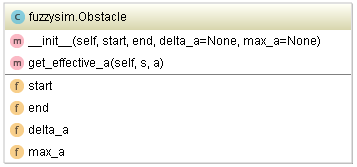
\includegraphics[scale=0.8]{3-6.png}
	\caption{ Структура класса fuzzisim.fuzzisim.Obstacle}
	% \label{fig:func:1}
\end{figure}

Поля класса \lstinline!fuzzisim.fuzzisim.Obstacle!:
\begin{itemize}
	\item \lstinline! start!. Начало участка, в метрах от препятствия.
	\item \lstinline! end!. Конец участка в метрах от препятствия.
	\item \lstinline! delta_a!. Константное ускорение на участке в метрах в секунду за секунду
	\item \lstinline! max_a!.  Максимальное ускорение на участкев метрах в секунду за секунду
\end{itemize}

Методы класса \lstinline!fuzzisim.fuzzisim.Obstacle!:
\begin{itemize}
	\item \lstinline! __init__(self, start, end, delta_a=None, max_a=None)!. Инициализирует поля объекта.
	\item \lstinline! get_effective_a(self, s, a)!.  Рассчитывает эффективное ускорение на данном участке пути. Входные аргументы: расстояние до препятствия в метрах, применяемое ускорение в метрах в секунду за секунду. Выходные параметры: рассчитанное эффективное ускорение в метрах в секунду за секунду.
\end{itemize}





\paragraph{fuzzisim.fuzzisim.CollisionError}
Исключение, возникающее при столкновении. Генерируется в \lstinline!fuzzisim.fuzzisim.Simulator.tick()!.


\begin{figure}[ht]
	\centering
	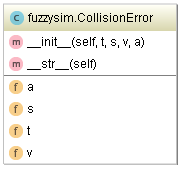
\includegraphics[scale=0.8]{3-7.png}
	\caption{ Структура класса fuzzisim.fuzzisim.CollisionError}
	% \label{fig:func:1}
\end{figure}

Поля класса \lstinline!fuzzisim.fuzzisim.CollisionError!:
\begin{itemize}
	\item \lstinline! t!. значения текущей метки времени в секундах.
	\item \lstinline! s!. расстояния до препятствия в метрах.
	\item \lstinline! v!. скорости в метрах в секунду.
	\item \lstinline! a!. ускорения в метрах в секунду за секунду.
\end{itemize}


Методы класса \lstinline!fuzzisim.fuzzisim.CollisionError!:
\begin{itemize}
	\item \lstinline! __init__(self, t,s,v,a)!. Инициализирует поля объекта.
	\item \lstinline! __str__(self)!.  Преобразует исключение в строку.
\end{itemize}



\subsubsection{ Блок моделирования нечетких алгоритмов }

Блок моделирования нечетких алгоритмов реализует разнообразные варианты нечетких алгоритмов, в частности Мамдани. Приведенные в нем реализации основаны на алгоритме Мамдани, и, в свою очередь, могут рассматриваться как основа для пользовательских реализаций контроллеров. Благодаря тому, что выбранный язык разработки является интерпретируемым, добавление новых реализаций не требует компилятора или другого подобного ПО, достаточно просто интерпретатора языка и текстового редактора.

Рассмотрим подробнее структуру блока. Он состоит из следующих классов:

\begin{itemize}
	\item \lstinline! fuzzisim.brake_controller.naive.Controller;!
	\item \lstinline! fuzzisim.brake_controller.custom_fuzzy.Controller;!
	\item \lstinline! fuzzisim.mamdani.MamdaniAlgorithm;!
	\item \lstinline! fuzzisim.mamdani.Rule;!
	\item \lstinline! fuzzisim.mamdani.Conclusion;!
	\item \lstinline! fuzzisim.mamdani.Cond;!
	\item \lstinline! fuzzisim.mamdani.FuzzyValue;!
	\item \lstinline! fuzzisim.mamdani.RectangleFuzzyValue;!
	\item \lstinline! fuzzisim.mamdani.IntervalFuzzyValue;!
	\item \lstinline! fuzzisim.mamdani.Membership;!
	\item \lstinline! fuzzisim.mamdani.Variable;!
	\item \lstinline! fuzzisim.mamdani.Term;!
	\item \lstinline! fuzzisim.mamdani.RectangleTerm;!
	\item \lstinline! fuzzisim.mamdani.IntervalTerm.!
\end{itemize}



\paragraph{fuzzisim.brake\_controller.naive.Controller}

Простой неадаптивный алгоритм торможения, используемый для калибровки и обучения нечетких алгоритмов. Основан на том, что при плавной остановке ускорение нарастает линейно до середины времени торможения, а максимальная его величина равна удвоенному ускорению при равнозамедленном движении. Ниже приведен код основного метода этого алгоритма.


\begin{figure}[ht]
	\centering
	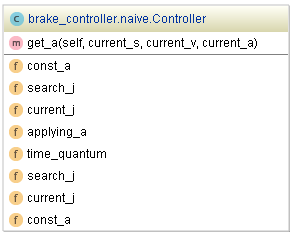
\includegraphics[scale=0.8]{3-8.png}
	\caption{ Структура класса fuzzisim.brake\_controller.naive.Controller}
	% \label{fig:func:1}
\end{figure}

Поля класса \lstinline!fuzzisim.brake_controller.naive.Controller!:
\begin{itemize}
	\item \lstinline! applying_a!. Текущее применяемое ускорение, в метрах в секунду за секунду.
	\item \lstinline! time_quantum!. Величина кванта времени, в секундах.
	\item \lstinline! search_j!. Модуль расчетного значения рывка, в метрах в секунду за секунду за секунду.
	\item \lstinline! current_j!. Текущее значение рывка, в метрах в секунду за секунду за секунду.
	\item \lstinline! const_a!. Ускорение необходимое для остановки при равнозамедленном движении.
\end{itemize}


Методы класса \lstinline!fuzzisim.brake_controller.naive.Controller!:
\begin{itemize}
	\item \lstinline! get_a(self, current_s, current_v, current_a)!. Возвращаетрассчетное ускорение для текущих расстояния, скорости и фактического ускорения.
\end{itemize}

\begin{lstlisting}[style=pythonstyle,caption={  }, label=lst:func:1]
def get_a(self, current_s, current_v, current_a):
   if self.search_j is None:
       self.const_a = -current_v ** 2 / (2 * current_s)
       time_a_const = 2 * current_s / current_v

       self.search_j = abs((self.const_a - current_a) * 2 / (time_a_const / 2))
       self.current_j = -self.search_j

   if self.current_j == -self.search_j:
       self.current_j = math.copysign(self.search_j, self.const_a * 2 - self.applying_a)

   self.applying_a += self.current_j * self.time_quantum

   return self.applying_a
\end{lstlisting}



%%%%%%%%%%%%%%%%%%%%%%%%%%%%%%%%%%%%%%%%%%%%%%%%%%%%%%%%%%%%%%%%%%%%%%%%%%%%%%%%%%%%%
\paragraph{fuzzisim.brake\_controller.custom\_fuzzy.Controller}
Адаптивный, настраиваемый алгоритм контроллера торможения на основе алгоритма Мамдани. Поддерживает треугольную и интервальную форму функций принадлежности, позволяет загружать термы и правила из конфигурационного json-файла.

Приведем пример конфигурационного файла для трех входных и трех выходных термов:
\begin{lstlisting}[style=pythonstyle,caption={  }, label=lst:func:1]
{
    "rules": [
        {
            "generated":1,
            "conds": [["S",0],["V",0]],
            "concs": [["A", 1]]
        },
        {
            "generated":1,
            "conds": [["S",0],["V",1]],
            "concs": [["A", 2]]
        },
        {
            "generated":1,
            "conds": [["S",0],["V",2]],
            "concs": [["A", 2]]
        },
        {
            "conds": [["S",1],["V",0]],
            "concs": [["A", 0]]
        },
        {
            "conds": [["S",1],["V",1]],
            "concs": [["A", 0]]
        },
        {
            "generated":1,
            "conds": [["S",1],["V",2]],
            "concs": [["A", 1]]
        },
        {
            "conds": [["S",2],["V",0]],
            "concs": [["A", 0]]
        },
        {
            "conds": [["S",2],["V",1]],
            "concs": [["A", 0]]
        },
        {
            "generated":1,
            "conds": [["S",2],["V",2]],
            "concs": [["A", 0]]
        }
    ],
    "S": {
        "max": 99.98,
        "min": 0.0493,
        "peaks": [
            16.704416666666667,
            50.01465,
            83.32488333333333
        ],
        "interval": 0
    },
    "A": {
        "min": 0.0,
        "max": 5,
        "interval": false,
        "peaks": [
            1,
            1.6,
            3.88
        ]
    },
    "V": {
        "max": 20.0,
        "min": 0.0009,
        "peaks": [
            3.334083333333333,
            10.000449999999999,
            16.666816666666666
        ],
        "interval": 0
    }}
\end{lstlisting}

Здесь поле rules задает набор нечетких правил. Каждое правило состоит из трех полей:
\begin{itemize}
	\item \lstinline! generated!. Флаг, показывающий, что поле сгенерировано автоматически;
	\item \lstinline! conds!. Список условий, каждое из которых является списком из двух элементов, имени переменной и номера терма соответственно;
	\item \lstinline! concs!. Список заключений, каждое из которых является списком из двух элементов, имени переменной и номера терма соответственно.
\end{itemize}

При работе алгоритма полагаем, что условия объединяются через AND.

Поле S описывает входную лингвистическую переменную расстояния до препятствия:
\begin{itemize}
	\item \lstinline! max!. Верхняя граница области значений лингвистической переменной, в метрах;
	\item \lstinline! min!. Нижняя граница области значений лингвистической переменной, в метрах;
	\item \lstinline! peaks!. Список пиков функции принадлежности (вершин треугольников треугольной функции, либо середин интервалов интервальных функций принадлежности), в метрах;
	\item \lstinline! interval!. Флаг, указывающий, является ли функция принадлежности интервальной.
\end{itemize}

Поле V описывает входную лингвистическую переменную скорости:
\begin{itemize}
	\item \lstinline! max!. Верхняя граница области значений лингвистической переменной, в метрах в секунду;
	\item \lstinline! min!. Нижняя граница области значений лингвистической переменной, в метрахв секунду;
	\item \lstinline! peaks!. Список пиков функции принадлежности (вершин треугольников треугольной функции, либо середин интервалов интервальных функций принадлежности), в метрах в секунду;
	\item \lstinline! interval!. Флаг, указывающий, является ли функция принадлежности интервальной.
\end{itemize}

Поле A описывает выходную лингвистическую переменную ускорения:
\begin{itemize}
	\item \lstinline! max!. Верхняя граница области значений лингвистической переменной, в метрах в секунду за секунду;
	\item \lstinline! min!. Нижняя граница области значений лингвистической переменной, в метрахв секундуза секунду;
	\item \lstinline! peaks!. Список пиков функции принадлежности (вершин треугольников треугольной функции, либо середин интервалов интервальных функций принадлежности), в метрах в секундуза секунду;
	\item \lstinline! interval!. Флаг, указывающий, является ли функция принадлежности интервальной.
\end{itemize}

\begin{figure}[ht]
	\centering
	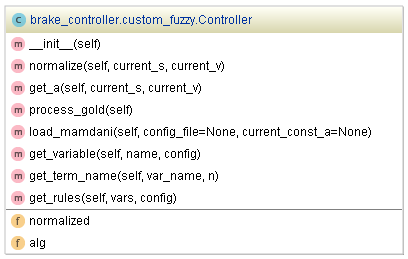
\includegraphics[scale=0.8]{3-9.png}
	\caption{ Структура класса fuzzisim.brake\_controller.custom\_fuzzy.Controller}
	% \label{fig:func:1}
\end{figure}

Поля класса \lstinline!fuzzisim.brake_controller.custom_fuzzy.Controller!:
\begin{itemize}
	\item \lstinline! normalized!. Флаг, указывающий, была ли проведена нормализация правил и  лингвистических переменных исходя из начальных скорости и расстояния.
	\item \lstinline! alg!. Экземпляр fuzzisim.mamdani.MamdaniAlgorithm, который используется для получения выходных значений.
\end{itemize}


Методы класса \lstinline!fuzzisim.brake_controller.custom_fuzzy.Controller!:
\begin{itemize}
	\item \lstinline! __init__(self) !— Инициализирует поля класса.
	\item \lstinline! normalize(self, current_s, current_v)!. Нормализует правила и лингвистические переменные. На вход принимает текущую скорость вметрах в секунду и расстояние в метрах.
	\item \lstinline! get_a(self, current_s, current_v)!. Возвращает расчетное значение ускорения в метрах в секунду за секунду. На вход принимает текущую скорость вметрах в секунду и расстояние в метрах.
	\item \lstinline! load_mamdani(self, config_file=None, current_const_a=None) !— Загружает лингвистические переменные и правила из файла и возвращает сконфигурированный экземпляр fuzzisim.mamdani.MamdaniAlgorithm.
	\item \lstinline! get_variable(self, name, config)!. Извлекает из конфигурационного объекта, конструирует  и возвращает экземпляр fuzzisim.mamdani.Variable, представляющий лингвистическую переменную.
	\item \lstinline! get_term_name(self, var_name, n)!.  Возвращает строку с именем терма. На вход принимает имя переменной и номер терма.
	\item \lstinline! get_rules(self, vars, config)!. Возвращает массив объектов fuzzisim.mamdani.Rule, представляющих лингвистические правила алгоритма Мамдани.
\end{itemize}



%%%%%%%%%%%%%%%%%%%%%%%%%%%%%%%%%%%%%%%%%%%%%%%%%%%%%%%%%%%%%%%%%%%%%%%%%%%%%%%%%%%%%
\paragraph{fuzzisim.mamdani.MamdaniAlgorithm}

Реализует алгоритм Мамдани в двух вариантах: классическом и ускоренном. Ускоренный вариант алгоритма Мамдани описан в [4]. Данная реализация этапа дефаззификации основана на том, что при интервальном задании выходной функции принадлежности появляется возможность подсчета центра масс не путем численного интегрирования, а путем сложения активированных интервалов выходной функции принадлежности, что позволяет уменьшить количество итераций в алгоритме дефаззификации на насколько порядков.

На рис. 3.8 показаны графики $V(t)^M$, $S(t)^M$ для классического и упрощенного вариантов реализации  алгоритма Мамдани в идеальных условиях – а, при введении временной инерционности системы торможения – б, при введении условий слабого сцепления платформы с дорогой на одном из участков.

Из сравнительного анализа результатов моделирования  видно, что алгоритмы нечеткого управления позволяют выполнить торможение в режиме, близком к эталонному. При этом графики классического и упрощенного вариантов реализации алгоритма Мамдани,
практически сливаются. Это говорит о том, что качество алгоритмов нечеткого контроллера при упрощенном варианте реализации не ухудшается. [4]

\begin{figure}[ht]
	\centering
	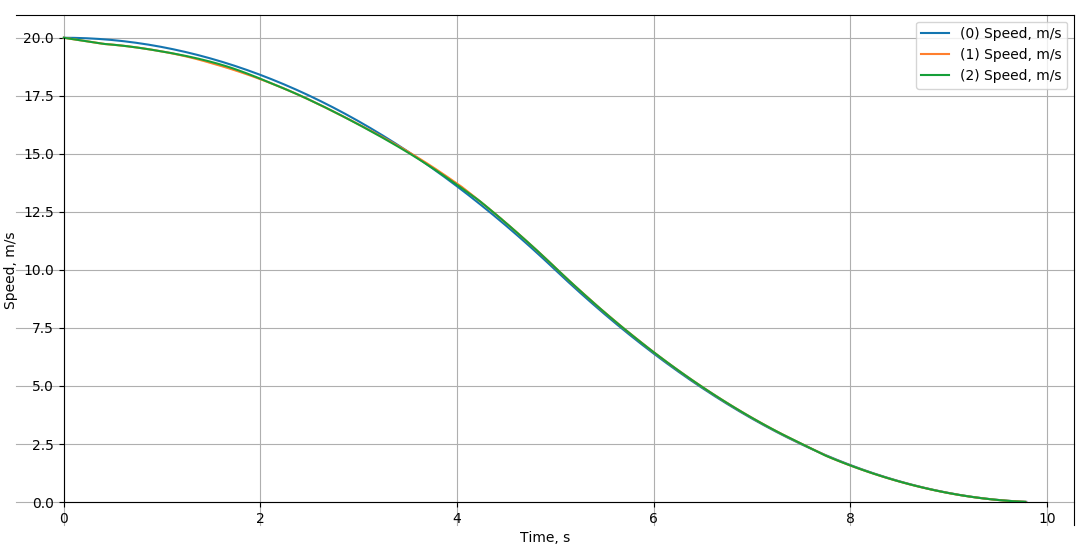
\includegraphics[scale=0.4]{3-10.png}
	\caption{ Графики скорости для экспериментов с эталонным, классическим алгоритмом Мамдани и ускоренным алгоритмом Мамдани. }
	% \label{fig:func:1}
\end{figure}

.

\begin{figure}[ht]
	\centering
	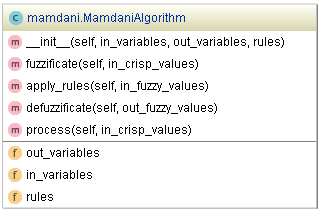
\includegraphics[scale=0.8]{3-11.png}
	\caption{ Структура класса fuzzisim.mamdani.MamdaniAlgorithm}
	% \label{fig:func:1}
\end{figure}

Поля класса \lstinline!fuzzisim.mamdani.MamdaniAlgorithm!:
\begin{itemize}
	\item \lstinline! out_variables!. Список объектов класса fuzzisim.mamdani.Variable, выходных лингвистических переменных.
	\item \lstinline! in_variables!.  Список объектов класса fuzzisim.mamdani.Variable, входных лингвистических переменных.
	\item \lstinline! rules !— Список объектов класса fuzzisim.mamdani.Rule, лингвистических правил алгоритма Мамдани.
\end{itemize}


Методы класса \lstinline!fuzzisim.mamdani.MamdaniAlgorithm!:
\begin{itemize}
	\item \lstinline! _init__(self, in_variables, out_variables, rules)!. Инициализирует поля объекта.
	\item \lstinline! fuzzificate(self, in_crisp_values)!. Фаззифицирует входные переменные. Получает на вход словарь конкретных значений входных переменных,  возвращает словарь с фаззифицированными  значениями fuzzisim.mamdani.FuzzyValue.
	\item \lstinline! apply_rules(self, in_fuzzy_values)!. Осуществляет агрегирование подусловий, активацию подзаключений и аккумулирование подзаключений. Получает на вход входные фаззифицированные значения, возвращает словарь с выходными фаззифицированными значениями.
	\item \lstinline! defuzzificate(self, out_fuzzy_values)!. Производит дефаззификацию. Деффазификация происходит по методу центра масс. На вход получает фаззифицированные значения выходных переменных, возвращает точные значения выходных переменных.
	\item \lstinline! process(self, in_crisp_values)!. Исполняет алгоритм в целом. На вход получает точные значения входных переменных, возвращает точные значения выходных переменных.
\end{itemize}

%%%%%%%%%%%%%%%%%%%%%%%%%%%%%%%%%%%%%%%%%%%%%%%%%%%%%%%%%%%%%%%%%%%%%%%%%%%%%%%%%%%%%
\paragraph{fuzzisim.mamdani.Rule}

Реализация лингвистического правила алгоритма Мамдани. Принимается, что условия объединены логическим AND.



\begin{figure}[ht]
	\centering
	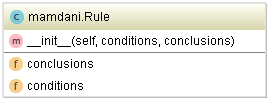
\includegraphics[scale=0.8]{3-12.png}
	\caption{ Структура класса fuzzisim.mamdani.Rule}
	% \label{fig:func:1}
\end{figure}

Поля класса \lstinline!fuzzisim.mamdani.Rule!:
\begin{itemize}
	\item \lstinline! conclusions!. Список объектов класса fuzzisim.mamdani.Conclusion, заключений алгоритма Мамдани.
	\item \lstinline! conditions!.  Список объектов класса fuzzisim.mamdani.Cond, условий алгоритма Мамдани.
\end{itemize}


Методы класса \lstinline!fuzzisim.mamdani.Rule!:
\begin{itemize}
	\item \lstinline! __init__(self, conditions, conclusions)!. Инициализирует поля объекта.
\end{itemize}



%%%%%%%%%%%%%%%%%%%%%%%%%%%%%%%%%%%%%%%%%%%%%%%%%%%%%%%%%%%%%%%%%%%%%%%%%%%%%%%%%%%%%
\paragraph{fuzzisim.mamdani.Conclusion}

Реализация заключения алгоритма Мамдани.

Поля класса \lstinline!fuzzisim.mamdani.Conclusion!:
\begin{itemize}
	\item \lstinline! variable!. Экземпляр класса \lstinline! fuzzisim.mamdani.Variable!, лингвистическая переменная алгоритма Мамдани.
	\item \lstinline! term!.   Экземпляр класса  \lstinline!fuzzisim.mamdani.Term!, терм лингвистической переменной алгоритма Мамдани.
\end{itemize}


Методы класса \lstinline!fuzzisim.mamdani.Conclusion!:
\begin{itemize}
	\item \lstinline! __init__(self, variable, term)!. Инициализирует поля объекта.
\end{itemize}


\begin{figure}[ht]
	\centering
	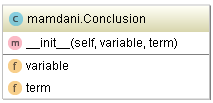
\includegraphics[scale=0.8]{3-13.png}
	\caption{ Структура класса fuzzisim.mamdani.Conclusion}
	% \label{fig:func:1}
\end{figure}


%%%%%%%%%%%%%%%%%%%%%%%%%%%%%%%%%%%%%%%%%%%%%%%%%%%%%%%%%%%%%%%%%%%%%%%%%%%%%%%%%%%%%
\paragraph{fuzzisim.mamdani.Cond}

Реализация условия алгоритма Мамдани.

\begin{figure}[ht]
	\centering
	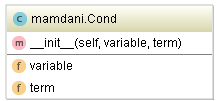
\includegraphics[scale=0.8]{3-14.png}
	\caption{ Структура класса fuzzisim.mamdani.Cond}
	% \label{fig:func:1}
\end{figure}

Поля класса \lstinline!fuzzisim.mamdani.Cond!:
\begin{itemize}
	\item \lstinline! variable!. Экземпляр класса  fuzzisim.mamdani.Variable, лингвистическая переменная алгоритма Мамдани.
	\item \lstinline! term!.   Экземпляр класса  fuzzisim.mamdani.Term, терм лингвистической переменной алгоритма Мамдани.
\end{itemize}


Методы класса \lstinline!fuzzisim.mamdani.Cond!:
\begin{itemize}
	\item \lstinline! __init__(self, variable, term)!. Инициализирует поля объекта.
\end{itemize}

\begin{lstlisting}[style=pythonstyle,caption={  }, label=lst:func:1]

\end{lstlisting}



%%%%%%%%%%%%%%%%%%%%%%%%%%%%%%%%%%%%%%%%%%%%%%%%%%%%%%%%%%%%%%%%%%%%%%%%%%%%%%%%%%%%%
\paragraph{fuzzisim.mamdani.FuzzyValue}

Базовая реализация нечеткого значения для классического алгоритма Мамдани.

\begin{figure}[ht]
	\centering
	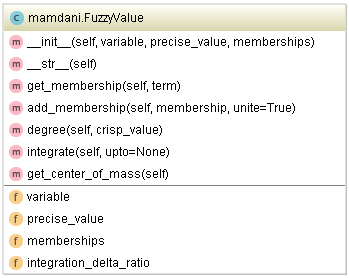
\includegraphics[scale=0.8]{3-15.png}
	\caption{ Структура класса fuzzisim.mamdani.FuzzyValue}
	% \label{fig:func:1}
\end{figure}

Поля класса \lstinline!fuzzisim.mamdani.FuzzyValue!:
\begin{itemize}
	\item \lstinline! variable!. Экземпляр класса  fuzzisim.mamdani.Variable, лингвистическая переменная алгоритма Мамдани.
	\item \lstinline! precise_value!.   Точное значение переменной.
	\item \lstinline! memberships!. Список экземпляров класса   fuzzisim.mamdani.Membership, признак принадлежности значения терму лингвистической переменной.
	\item \lstinline! integration_delta_ratio!.   Коэффициент шага интегрирования для классической дефаззификации.
\end{itemize}


Методы класса \lstinline!fuzzisim.mamdani.FuzzyValue!:
\begin{itemize}
	\item \lstinline! __init__(self, variable, precise_value, memberships)!. Инициализирует поля класса.
	\item \lstinline! __str__(self)!.   Преобразует объект в строку для дальнейшего вывода.
	\item \lstinline! get_membership(self, term)!. Возвращает объект класса \lstinline!fuzzisim.mamdani.Membership!, степень принадлежности значения данному терму.
	\item \lstinline! add_membership(self, membership, unite=True)!. Устанавливает принадлежность данному терма. Если аргумент \lstinline!unite! равен True, то в случае существования принадлежности данному терму будет произведено объединение принадлежностей по \lstinline!max()!. В противном случае будет возбуждено исключение.
	\item \lstinline! degree(self, crisp_value)!.  Возвращает активированное значение при аккумуляции заключений.
	\item \lstinline! integrate(self, upto=None)!. Производит классическое интегрирование по области значений переменной с шагом, определяемым \lstinline!integration_delta_ratio!. Если установлен аргумент \lstinline!upto!, останавливает интегрирование при достижении значения равного \lstinline!upto!, возвращает полученное значение, а также соответствующее ему значение лингвистической переменной
	\item \lstinline! get_center_of_mass(self)!. Находит центр масс используя метод \lstinline!integrate!. Возвращает скалярное значения центра масс.
\end{itemize}




%%%%%%%%%%%%%%%%%%%%%%%%%%%%%%%%%%%%%%%%%%%%%%%%%%%%%%%%%%%%%%%%%%%%%%%%%%%%%%%%%%%%%
\paragraph{fuzzisim.mamdani.IntervalFuzzyValue}

Дочерний класс fuzzisim.mamdani.FuzzyValue. Реализует нечеткое значение с интервальным заданием функции принадлежности для ускоренной дефаззификации. Накладывает ограничения на выходную лингвистическую переменную:

\begin{itemize}
	\item \lstinline! !Термы выходной переменной должны быть заданы на непрерывном интервале;
	\item \lstinline! !Термы выходной переменной должны отсортированы в порядке следования по области определения.
\end{itemize}

\begin{figure}[ht]
	\centering
	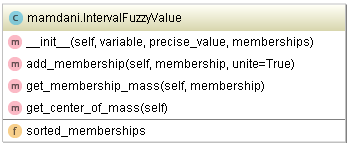
\includegraphics[scale=0.8]{3-16.png}
	\caption{ Структура класса fuzzisim.mamdani.IntervalFuzzyValue}
	% \label{fig:func:1}
\end{figure}

Поля класса \lstinline!fuzzisim.mamdani.IntervalFuzzyValue!:
\begin{itemize}
	\item \lstinline! sorted_memberships!. Список экземпляров класса   fuzzisim.mamdani.Membership, сортированный по началу области определения соответствующего терма.
\end{itemize}


Методы класса \lstinline!fuzzisim.mamdani.IntervalFuzzyValue!:
\begin{itemize}
	\item \lstinline! __init__(self, variable, precise_value, memberships)!. Инициализирует поля класса.
	\item \lstinline! get_membership_mass(self, membership)!. Возвращает вес принадлежности к терму: произведение ширины терма на степень принадлежности к терму.
	\item \lstinline! add_membership(self, membership, unite=True)!. Устанавливает принадлежность данному терма. Если аргумент unite равен True, то в случае существования принадлежности данному терму будет произведено объединение принадлежностей по max(). В противном случае будет возбуждено исключение. После добавления принадлежности.
	\item \lstinline! get_center_of_mass(self)!. Производит дефаззификацию нечеткого значения по ускоренному алгоритму. Для этого вычисляются массы каждой принадлежности к каждому терму и суммируются для получения полной массы полигона. Затем итеративно в счетчике суммируются массы принадлежностей до тех пор, пока масса суммы не станет больше половины массы всего полигона. Затем от полученного точного значения отнимается доля ширины последней принадлежности, пропорциональна превышению суммы надо половиной массы полигона.
\end{itemize}

\begin{lstlisting}[style=pythonstyle,caption={  }, label=lst:func:1]
def get_center_of_mass(self):
  masses = [0] * len(self.sorted_memberships)
  total_mass = 0

  for i, m in enumerate(self.sorted_memberships):
     masses[i] = self.get_membership_mass(m)
     total_mass += masses[i]

  if total_mass == 0:
		result = (self.variable.max + self.variable.min)/2
     return result

  half_mass = total_mass / 2
  center = 0

  for i, v in enumerate(masses):
     half_mass -= v

     if half_mass <= 0:
          ratio = 1 - abs(half_mass / v)
  		part=ratio*self.sorted_memberships[i].term.width
center += part

        return center

     center += self.sorted_memberships[i].term.width
\end{lstlisting}








%%%%%%%%%%%%%%%%%%%%%%%%%%%%%%%%%%%%%%%%%%%%%%%%%%%%%%%%%%%%%%%%%%%%%%%%%%%%%%%%%%%%%
\paragraph{fuzzisim.mamdani.RectagleFuzzyValue}

Дочерний класс\lstinline! fuzzisim.mamdani.IntervalFuzzyValue!. Реализует нечеткое значение с прямоугольным заданием функции принадлежности для ускоренной дефаззификации. Переопределяет метод \lstinline!get_membership_mass!, учитывая высоту терма.

\begin{figure}[ht]
	\centering
	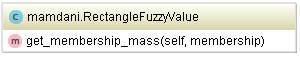
\includegraphics[scale=0.8]{3-17.png}
	\caption{ Структура класса fuzzisim.mamdani.RectagleFuzzyValue}
	% \label{fig:func:1}
\end{figure}


Методы класса \lstinline!fuzzisim.mamdani.RectagleFuzzyValue!:
\begin{itemize}
	\item \lstinline! get_membership_mass(self, membership)!. Возвращает вес принадлежности к терму: произведение ширины терма на степень принадлежности к терму.
\end{itemize}






%%%%%%%%%%%%%%%%%%%%%%%%%%%%%%%%%%%%%%%%%%%%%%%%%%%%%%%%%%%%%%%%%%%%%%%%%%%%%%%%%%%%%
\paragraph{ fuzzisim.mamdani.Membership}

Реализует абстракцию принадлежности значения к терму.

\begin{figure}[ht]
	\centering
	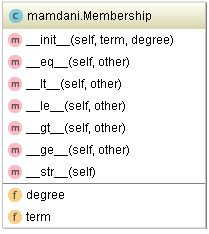
\includegraphics[scale=0.8]{3-18.png}
	\caption{ Структура класса  fuzzisim.mamdani.Membership}
	% \label{fig:func:1}
\end{figure}

Поля класса \lstinline! fuzzisim.mamdani.Membership!:
\begin{itemize}
	\item \lstinline! degree!. Степень принадлежности к терму. Число от 0 до 1 включительно.
	\item \lstinline! term!.   Экземпляр класса  fuzzisim.mamdani.Term, терм лингвистической переменной алгоритма Мамдани.
\end{itemize}


Методы класса \lstinline! fuzzisim.mamdani.Membership!:
\begin{itemize}
	\item \lstinline! __init__(self, term, degree)!. Инициализирует поля объекта.
	\item \lstinline!  __eq__(self, other)!. Магический метод “равно” объектов класса fuzzisim.mamdani.Membership
	\item \lstinline! __lt__(self, other)!. Магический метод “меньше, чем” объектов класса fuzzisim.mamdani.Membership
	\item \lstinline! __le__(self, other)!. Магический метод “меньше или равно” объектов класса fuzzisim.mamdani.Membership
	\item \lstinline! __gt__(self, other)!. Магический метод “больше, чем” объектов класса fuzzisim.mamdani.Membership
	\item \lstinline! __ge__(self, other)!. Магический метод “больше или равно” объектов класса fuzzisim.mamdani.Membership
	\item \lstinline! __str__(self)!. Магический метод преобразования в строку объектов класса fuzzisim.mamdani.Membership
\end{itemize}







%%%%%%%%%%%%%%%%%%%%%%%%%%%%%%%%%%%%%%%%%%%%%%%%%%%%%%%%%%%%%%%%%%%%%%%%%%%%%%%%%%%%%
\paragraph{fuzzisim.mamdani.Variable}
Реализует лингвистическую переменную алгоритма Мамдани. Позволяет получить нечеткое значение на основе конкретного.

\begin{figure}[ht]
	\centering
	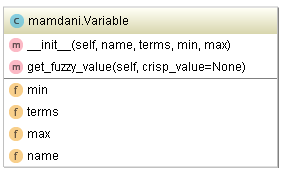
\includegraphics[scale=0.8]{3-19.png}
	\caption{ Структура класса fuzzisim.mamdani.Variable}
	% \label{fig:func:1}
\end{figure}

Поля класса \lstinline!fuzzisim.mamdani.Variable!:
\begin{itemize}
	\item \lstinline! min!. Нижняя граница области определения лингвистической переменной, скаляр.
	\item \lstinline! max!. Верхняя граница области определения лингвистической переменной, скаляр.
	\item \lstinline! terms!.   Список экземпляров класса  fuzzisim.mamdani.Term, задает термы лингвистической переменной алгоритма Мамдани.
	\item \lstinline! name!. Имя лингвистической переменной алгоритма Мамдани.
\end{itemize}


Методы класса \lstinline!fuzzisim.mamdani.Variable!:
\begin{itemize}
	\item \lstinline! __init__(self, name, terms, min, max)!. Инициализирует поля объекта.
	\item \lstinline!  get_fuzzy_value(self, crisp_value=None)!. Возвращает нечеткое значение fuzzisim.mamdani.FuzzyValue данной переменной, соответствующее скалярному значению аргумента функции.
\end{itemize}





%%%%%%%%%%%%%%%%%%%%%%%%%%%%%%%%%%%%%%%%%%%%%%%%%%%%%%%%%%%%%%%%%%%%%%%%%%%%%%%%%%%%%
\paragraph{fuzzisim.mamdani.Term}

Базовый класс, реализует терм лингвистической переменной классического алгоритма Мамдани с трапецеидальной функцией принадлежности.

\begin{figure}[ht]
	\centering
	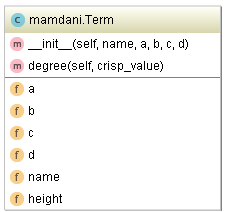
\includegraphics[scale=0.8]{3-20.png}
	\caption{ Структура класса fuzzisim.mamdani.Term}
	% \label{fig:func:1}
\end{figure}

Поля класса \lstinline!fuzzisim.mamdani.Term!:
\begin{itemize}
	\item \lstinline! a!. Начало области определения терма, скаляр.
	\item \lstinline! b!. Начало интервала, где значение функции принадлежности терма становится равным высоте терма, скаляр.
	\item \lstinline! c!. Конец интервала, где значение функции принадлежности терма становится равным высоте терма, скаляр.
	\item \lstinline! d!.   Конец области определения терма, скаляр.
	\item \lstinline! height!. Высота терма, максимальное значение функции принадлежности терма.
	\item \lstinline! name!. Имя терма лингвистической переменной алгоритма Мамдани.
\end{itemize}


Методы класса \lstinline!fuzzisim.mamdani.Term!:
\begin{itemize}
	\item \lstinline! __init__(self, name, a, b, c, d)!. Инициализирует поля объекта.
	\item \lstinline! degree(self, crisp_value)!. Возвращает степень принадлежности скалярного значения терму.
\end{itemize}


%%%%%%%%%%%%%%%%%%%%%%%%%%%%%%%%%%%%%%%%%%%%%%%%%%%%%%%%%%%%%%%%%%%%%%%%%%%%%%%%%%%%%
\paragraph{fuzzisim.mamdani.RectangleTerm}

Реализует терм лингвистической переменной ускоренного алгоритма Мамдани с прямоугольной функцией принадлежности. Нахождение принадлежности значения этому терму вычислительно проще, чем классическому, благодаря тому, что значение степени принадлежности дискретно и может быть либо 0, либо 1.

Очевидно, что данный способ сочетает в себе черты классического ( с трапецеидальным заданием функций принадлежностей) и упрощенного алгоритма нечеткого вывода, где в результате обработки правил получаем и обрабатываем константы Ci .

Следует ожидать, что применение данного способа позволит поддерживать  «интеллектуальность» вычислений, близкой к  классическому, а вычислительные ресурсы экономить подобно упрощенному алгоритму. [4]

\begin{figure}[ht]
	\centering
	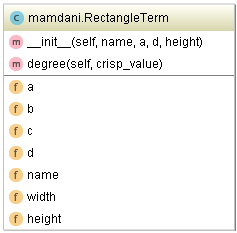
\includegraphics[scale=0.8]{3-21.png}
	\caption{ Структура класса fuzzisim.mamdani.RectangleTerm}
	% \label{fig:func:1}
\end{figure}

Поля класса \lstinline!fuzzisim.mamdani.RectangleTerm!:
\begin{itemize}
	\item \lstinline! a!. Начало области определения терма, скаляр.
	\item \lstinline! d!. Конец области определения терма, скаляр.
	\item \lstinline! width!. Ширина области определения терма, скаляр.
	\item \lstinline! height!. Высота терма, максимальное значение функции принадлежности терма.
	\item \lstinline! name!. Имя терма лингвистической переменной алгоритма Мамдани.
\end{itemize}


Методы класса \lstinline!fuzzisim.mamdani.RectangleTerm!:
\begin{itemize}
	\item \lstinline! __init__(self, name, a, d, height)!. Инициализирует поля объекта.
	\item \lstinline! degree(self, crisp_value)!. Возвращает степень принадлежности скалярного значения терму.
\end{itemize}



%%%%%%%%%%%%%%%%%%%%%%%%%%%%%%%%%%%%%%%%%%%%%%%%%%%%%%%%%%%%%%%%%%%%%%%%%%%%%%%%%%%%%
\paragraph{fuzzisim.mamdani.IntervalTerm}

Реализует терм лингвистической переменной ускоренного алгоритма Мамдани с интервальной функцией принадлежности. Дочерний класс fuzzisim.mamdani.RectangleTerm. Является прямоугольным термом с высотой, которая всегда равна 1.

\begin{figure}[ht]
	\centering
	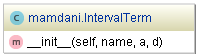
\includegraphics[scale=0.8]{3-22.png}
	\caption{ Структура класса fuzzisim.mamdani.IntervalTerm}
	% \label{fig:func:1}
\end{figure}



Методы класса \lstinline!fuzzisim.mamdani.IntervalTerm!:
\begin{itemize}
	\item \lstinline! __init__(self, name, a, d)!. Инициализирует поля объекта.  Устанавливает высоту родительского класса в 1.
\end{itemize}

\subsection{Верификация проекта и анализ полученных результатов}

Верификация проверяет соответствие одних создаваемых в ходе разработки и сопровождения ПО артефактов другим, ранее созданным или используемым в качестве исходных данных, а также соответствие этих артефактов и процессов их разработки правилам и стандартам. В частности, верификация проверяет соответствие между нормами стандартов, описанием требований (техническим заданием) к ПО, проектными решениями, исходным кодом, пользовательской документацией и функционированием самого ПО. Кроме того, проверяется, что требования, проектные решения, документация и код оформлены в соответствии с нормами и стандартами, принятыми в данной стране, отрасли и организации при разработке ПО, а также — что при их создании выполнялись все указанные в стандартах операции, в нужной последовательности. Обнаруживаемые при верификации ошибки и дефекты являются расхождениями или противоречиями между несколькими из перечисленных документов, между документами и реальной работой программы, между нормами стандартов и реальным процессами разработки и сопровождения ПО. При этом принятие решения о том, какой именно документ подлежит исправлению (может быть, и оба) является отдельной задачей.

Тестирование (testing) является методом верификации, в рамках которого результаты работы тестируемой системы или компонента в ситуациях из выделенного конечного набора проверяются на соответствие проектным решениям, требованиям, общим задачам проекта, в рамках которого эта система разрабатывается или сопровождается. Ситуации, в которых выполняется тестирование, называют тестовыми ситуациями (test situations, test purposes), а процедуры, описывающие процесс создания этих ситуаций и проверки, которые необходимо выполнить над полученными результатами, — тестами.

Тестирование, как и верификация вообще, служит для поиска ошибок или дефектов и для оценки качества ПО. Эффективность решения обеих этих задач во многом определяется тем, какой именно набор тестовых ситуаций выбран для проведения тестирования. Чтобы иметь некоторые гарантии аккуратности полученных в ходе тестирования оценок качества, необходимо выбирать тестовые ситуации систематическим образом, в соответствии с основными задачами и рисками проекта. Правила, определяющие набор необходимых тестовых ситуаций, называют критериями полноты (или адекватности) тестирования (test adequacy criteria) [200- 202]. Обычно такой критерий использует разбиение всех возможных при работе проверяемого ПО ситуаций на некоторые классы эквивалентности, такие, что ситуации из одного класса достаточно похожи друг на друга и работа ПО в них не должна отличаться сколь-нибудь значительным образом.

Классификация видов тестирования достаточно сложна, потому что может проводиться по нескольким разным аспектам.  Самое распространенная классификация — классификация по уровню или масштабу проверяемых элементов системы. По этому критерию оно делится на следующие виды:

\begin{itemize}
	\item Модульное или компонентное (unit testing, component testing) — проверка корректности работы отдельных компонентов системы, выполнения ими своих функций и предполагаемых проектом характеристик.
	\item Интеграционное (integration testing) — проверка корректности взаимодействий внутри отдельных групп компонентов.
	\item Системное (system testing) — проверка работы системы в целом, выполнения ею своих основных функций, с использованием определенных ресурсов, в окружении с заданными характеристиками.
\end{itemize}

В данном проекте применялось как ручное, так и модульное тестирование. Автоматическими модульными тестами покрыта наиболее важная часть системы — реализация классического и ускоренных алгоритмов Мамдани.

\subsubsection{Верификация реализации классического алгоритма Мамдани. }

В качестве тестового набора выбрав следующие термы и правила, а также четкие значения входных переменных:

\begin{lstlisting}[style=pythonstyle,caption={  }, label=lst:func:1]
As = Term('As', 0, 0, 3, 5)
Al = Term('Al', 3, 6, inf, inf)
A = Variable('A', [As, Al], 0, 10)

Bs = Term('Bs', 0, 0, 3, 6)
Bl = Term('Bl', 4, 6, inf, inf)
B = Variable('B', [Bs, Bl], 0, 10)

Ws = Term('Ws', 0, 0, 1, 3)
Wm = Term('Wm', 2, 4, 6, 8)
Wl = Term('Wl', 6, 8, inf, inf)
W = Variable('W', [Ws, Wm, Wl], 0, 10)

in_variables = [A, B]

out_variables = [W, ]

rules = [
  Rule([Cond(A, As), Cond(B, Bs)], [Cond(W, Ws)]),
  Rule([Cond(A, As), Cond(B, Bl)], [Cond(W, Wm)]),
  Rule([Cond(A, Al), Cond(B, Bs)], [Cond(W, Wm)]),
  Rule([Cond(A, Al), Cond(B, Bl)], [Cond(W, Wl)]),
]

in_crisp_values = {'A': 4, 'B': 5}
\end{lstlisting}

Эталонные нечеткие значения входных переменных, которые должны получиться в результате фаззификации:

\begin{lstlisting}[style=pythonstyle,caption={  }, label=lst:func:1]
["FuzzyValue(A, 4.00, ['As(0.50)', 'Al(0.33)'])", "FuzzyValue(B, 5.00, ['Bs(0.33)', 'Bl(0.50)'])"]
\end{lstlisting}

Эталонные нечеткие значения выходных переменных, которые должны получиться в результате применения правил:

\begin{lstlisting}[style=pythonstyle,caption={  }, label=lst:func:1]
["FuzzyValue(W, 0.00, ['Wl(0.33)', 'Wm(0.50)', 'Ws(0.33)'])"]
\end{lstlisting}

Эталонные четкие значения выходных переменных, которые должны получиться в результате применения правил: 5,0

\subsubsection{Верификация реализации дефаззификации ускоренного алгоритма Мамдани с интервальным заданием функций принадлежности термов }

В качестве тестового набора выступают следующие термы, лингвистические переменные и степени принадлежностей:

\begin{lstlisting}[style=pythonstyle,caption={  }, label=lst:func:1]
Its = [
   IntervalTerm('I0', 0, 0.5),
   IntervalTerm('I1', 0.5, 1),
   IntervalTerm('I2', 1, 2.5),
   IntervalTerm('I3', 2.5, 4),
   IntervalTerm('I4', 4, 6),
   IntervalTerm('I5', 6, 7.2),
   IntervalTerm('I6', 7.2, 9),
   IntervalTerm('I7', 9, 9.5),
   IntervalTerm('I8', 9.5, 10),
]
I = Variable('I', Its, 0, 10)

degrees = [1, 1, 0.6, 0.6, 0.6, 0.6, 0.6, 0.6, 0.6, ]
Imemberships = {"I%d" % i: Membership(Its[i], v) for i, v in enumerate(degrees)}
ifv = IntervalFuzzyValue(I, None, Imemberships)
\end{lstlisting}


Эталонное четкое значение выходной переменной, которое должно получиться в результате применения правил равно 4,6666

\subsubsection{Верификация реализации дефаззификации ускоренного алгоритма Мамдани с прямоугольным заданием функций принадлежности термов }

В качестве тестового набора выступают следующие термы, лингвистические переменные и степени принадлежностей:

\begin{lstlisting}[style=pythonstyle,caption={  }, label=lst:func:1]
Rts = [
   RectangleTerm('R0', 0, 0.5, 0.6),
   RectangleTerm('R1', 0.5, 1, 0.6),
   RectangleTerm('R2', 1, 2.5, 0.6),
   RectangleTerm('R3', 2.5, 4, 0.6),
   RectangleTerm('R4', 4, 6, 1),
   RectangleTerm('R5', 6, 7.2, 0.6),
   RectangleTerm('R6', 7.2, 9, 0.6),
   RectangleTerm('R7', 9, 9.5, 1),
   RectangleTerm('R8', 9.5, 10, 1),
]
R = Variable('R', Rts, 0, 10)
degrees = [1, 1, 0.6, 0.6, 0.6, 0.6, 0.6, 0.6, 0.6, ]
Rmemberships = {"R%d" % i: Membership(Rts[i], v) for i, v in enumerate(degrees)}
rfv = RectangleFuzzyValue(R, None, Rmemberships)
\end{lstlisting}

Эталонное четкое значение выходной переменной, которое должно получиться в результате применения правил равно 5,0


\subsubsection{ерификация уменьшения времени выполнения ускоренных алгоритмов Мамдани по сравнению с классическим }

Для верификации уменьшения времени выполнения производится выполнение 10000 итераций каждой версии алгоритма с тестовыми наборами, указанными в пункте 3.3.2.

\begin{lstlisting}[style=pythonstyle,caption={  }, label=lst:func:1]
iterations = 10000
start = time.time()
for i in range(0, iterations):
   in_fuzzy_values = alg.fuzzificate(in_crisp_values)
print("%d alg.fuzzificate takes %.1f ms" % (iterations, 1000 * (time.time() - start)))
start = time.time()
for i in range(0, iterations):
   out_fuzzy_values = alg.apply_rules(in_fuzzy_values)
print("%d alg.apply_rules takes %.1f ms" % (iterations, 1000 * (time.time() - start)))
start = time.time()
for i in range(0, iterations):
   out_crisp_values = alg.defuzzificate(out_fuzzy_values)
print("%d alg.defuzzificate takes %.1f ms" % (iterations, 1000 * (time.time() - start)))
start = time.time()
for i in range(0, iterations):
   center = ifv.get_center_of_mass()
print("%d ifv.get_center_of_mass takes %.1f ms" % (iterations, 1000 * (time.time() - start)))
start = time.time()
for i in range(0, iterations):
   center = rfv.get_center_of_mass()
print("%d rfv.get_center_of_mass takes %.1f ms" % (iterations, 1000 * (time.time() - start)))
\end{lstlisting}